\documentclass[10pt]{article}\usepackage[]{graphicx}\usepackage[]{color}
%% maxwidth is the original width if it is less than linewidth
%% otherwise use linewidth (to make sure the graphics do not exceed the margin)
\makeatletter
\def\maxwidth{ %
  \ifdim\Gin@nat@width>\linewidth
    \linewidth
  \else
    \Gin@nat@width
  \fi
}
\makeatother

\definecolor{fgcolor}{rgb}{0.345, 0.345, 0.345}
\newcommand{\hlnum}[1]{\textcolor[rgb]{0.686,0.059,0.569}{#1}}%
\newcommand{\hlstr}[1]{\textcolor[rgb]{0.192,0.494,0.8}{#1}}%
\newcommand{\hlcom}[1]{\textcolor[rgb]{0.678,0.584,0.686}{\textit{#1}}}%
\newcommand{\hlopt}[1]{\textcolor[rgb]{0,0,0}{#1}}%
\newcommand{\hlstd}[1]{\textcolor[rgb]{0.345,0.345,0.345}{#1}}%
\newcommand{\hlkwa}[1]{\textcolor[rgb]{0.161,0.373,0.58}{\textbf{#1}}}%
\newcommand{\hlkwb}[1]{\textcolor[rgb]{0.69,0.353,0.396}{#1}}%
\newcommand{\hlkwc}[1]{\textcolor[rgb]{0.333,0.667,0.333}{#1}}%
\newcommand{\hlkwd}[1]{\textcolor[rgb]{0.737,0.353,0.396}{\textbf{#1}}}%

\usepackage{framed}
\makeatletter
\newenvironment{kframe}{%
 \def\at@end@of@kframe{}%
 \ifinner\ifhmode%
  \def\at@end@of@kframe{\end{minipage}}%
  \begin{minipage}{\columnwidth}%
 \fi\fi%
 \def\FrameCommand##1{\hskip\@totalleftmargin \hskip-\fboxsep
 \colorbox{shadecolor}{##1}\hskip-\fboxsep
     % There is no \\@totalrightmargin, so:
     \hskip-\linewidth \hskip-\@totalleftmargin \hskip\columnwidth}%
 \MakeFramed {\advance\hsize-\width
   \@totalleftmargin\z@ \linewidth\hsize
   \@setminipage}}%
 {\par\unskip\endMakeFramed%
 \at@end@of@kframe}
\makeatother

\definecolor{shadecolor}{rgb}{.97, .97, .97}
\definecolor{messagecolor}{rgb}{0, 0, 0}
\definecolor{warningcolor}{rgb}{1, 0, 1}
\definecolor{errorcolor}{rgb}{1, 0, 0}
\newenvironment{knitrout}{}{} % an empty environment to be redefined in TeX

\usepackage{alltt}
\usepackage[top=0.5in, left=0.5in, right=0.5in, bottom=0.5in]{geometry}

\usepackage{float, amsmath}
\usepackage{tikz}
\usetikzlibrary{shapes,arrows}
\usetikzlibrary{positioning}
\usepackage{float, amsmath}

\usepackage[hyphens]{url}
\usepackage{enumerate}
\usepackage[sort, numbers]{natbib}
\usepackage{sidecap}

\setlength{\bibsep}{0.0pt}
%\usepackage[
%  natbib = true,
%    backend=bibtex,
%    isbn=false,
%    url=false,
%    doi=false,
%    eprint=false,
%    style=numeric,
%    sorting=nyt,
%    sortcites = true
%]{biblatex}
%\bibliography{CT_Pipeline_l}
%\bibliography{CT_Skull_Stripping}


\usepackage{subfig}










%\usepackage[all]{hypcap}
\IfFileExists{upquote.sty}{\usepackage{upquote}}{}
\begin{document}
\renewcommand{\thesubfigure}{\Alph{subfigure}}

\vspace{-1cm}
\paragraph*{Introduction}
Computed Tomography (CT) imaging of the brain is commonly used in diagnostic settings.  Although CT scans are primarily used in clinical practice, they are increasingly used in research.  A fundamental processing step in brain imaging research is brain extraction, which is the process of separating the brain tissue from all other tissues. Methods for brain extraction in head CT images has been informally proposed \citep{able, rorden_age-specific_2012}, but never formally validated.

Our goal is to systematically analyze the performance of the brain extraction tool (BET) \citep{smith_fast_2002}, a function of the FMRIB software library (FSL) \citep{jenkinson_fsl_2012}, on head CT images of patients with intracranial hemorrhage by varying parameters of BET and the use of smoothing after performing CT-specific preprocessing, and quantitatively comparing the results to the manual gold standard.

\vspace{-0.4cm}
\paragraph*{Methods}
Nineteen images from 16 patients with intracranial hemorrhage were selected from 13 different MISTIE (Minimally Invasive Surgery plus recombinant-tissue plasminogen activator for Intracerebral Evacuation) stroke trial centers. After NIfTI conversion, the data is thresholded to tissue ranges of $0$-$100$ Hounsfield units (HU).  In one variant of the processing pipeline, the data was smoothed using a Gaussian kernel ($\sigma=1$mm); in the other, the data was not smoothed.  BET was then applied to the image using 3 different fractional intensity (FI) values: $0.01$, $0.1$, or $0.35$ and then holes in the brain mask produced by BET were filled.
For validation purposes, intracranial masks were manually created for all image volumes by expert CT readers.  The resulting brain tissue masks were quantitatively compared to the manual segmentations using sensitivity, specificity, accuracy, and the Dice Similarity Index (DSI).  Brain extraction across smoothing and FI thresholds were compared using the Wilcoxon signed-rank test.

\vspace{-0.4cm}
\paragraph*{Results}
Figure~\ref{fig:metrics}\protect\subref*{unsmoothed} illustrates the performance of each variation of the BET pipeline.  The pipelines using smoothing (top) perform better than the unsmoothed pipelines (bottom) on all measures except specificity (all $p < 0.01$, uncorrected).  We also note that BET performs poorly on some scans without smoothing.  Figure~\ref{fig:metrics}\protect\subref*{smoothed} displays the performance for brain extraction for the pipelines using smoothed images. 

Using an FI of $0.01$ or $0.1$ performed better than $0.35$; thus, we focused and compared results for these values of FI only for the case when BET was applied to smoothed images.  Using an FI of $0.01$ had a higher median sensitivity ($0.9921$) than an FI of $0.1$ ($0.9905$, $p< 0.001$), lower specificity ($0.9979$ vs. $0.998$; $p< 0.001$), with no difference in accuracy ($0.9971$ vs. $0.9971$; $p= 0.134$) or DSI ($0.9894$ vs. $0.9896$; $p= 0.066$).  Overall, regardless of p-values, these measures are all very high, indicating that multiple choices of parameters work well for brain extraction after CT image processing.

\vspace{-0.5cm}
\begin{SCfigure}[][h]
  \subfloat{
  \label{unsmoothed}
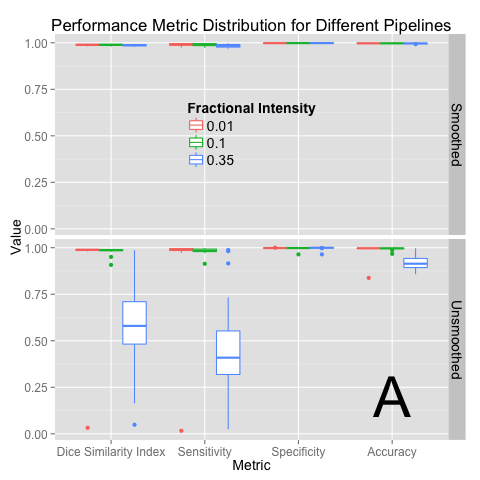
\includegraphics[width=.33\textwidth]{figure/CT_Skull_Stripping_Figure2.png}
}
\hfill
  \subfloat{
  \label{smoothed}
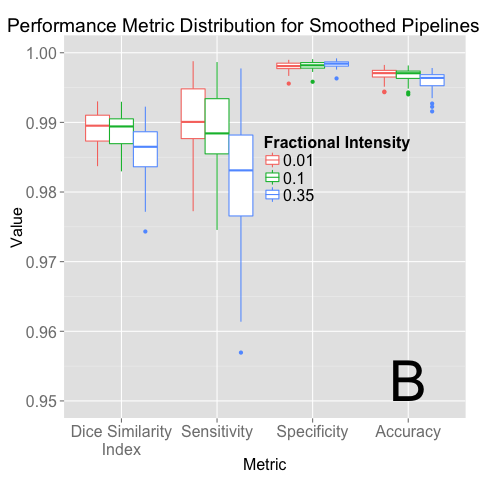
\includegraphics[width=.33\textwidth]{figure/CT_Skull_Stripping_Figure2b.png}
}
\caption{{\bf Performance Metric Distribution for Different Pipelines.} Panel~\protect\subref*{unsmoothed} displays boxplots for performance measures when running the pipeline with different FI, using smoothed data (top) or unsmoothed data (bottom).   Using smoothed data improves performance in performance metrics.  Panel~\protect\subref*{smoothed} presents the smoothed data only-- using an FI of $0.01$ and $0.1$ perform better than $0.35$ in all categories other than specificity. Based on all metrics, we recommend smoothing and an FI of $0.01$.}
\label{fig:metrics}
\end{SCfigure}

\vspace{-0.5cm}
\paragraph*{Conclusion}
We have introduced the first validated automated brain extraction pipeline for head CT images.  A novel finding is that smoothing the data using a conservative smoother ($1$mm Gaussian kernel) and using an FI of $0.01$ or $0.1$ provides good brain extraction for the sample studied.  These choices make a large difference in the performance of the algorithms and have not been previously reported in the literature.  The research presented here is fully reproducible and we provide ready-to-use software for CT brain extraction (see \url{http://bit.ly/CTBET_RCODE}). Our software is readily available to all users as it is based on open-source, free programs (FSL and R).


\vspace{-0.4cm}
\paragraph*{Sources of Funding}
The project described and data used were supported by the NIH grants RO1EB012547, T32AG000247, R01NS046309, RO1NS060910, RO1NS085211, R01NS046309, U01NS080824, U01NS080824 and U01NS062851 and RO1MH095836.

\vspace{-0.25cm}
\subsubsection*{References}
\renewcommand\refname{\vskip -1cm}
\bibliographystyle{abbrv}
\bibliography{CT_Skull_Stripping_Abstract}

%\printbibliography



\end{document}
